\documentclass[11pt,a4paper]{book}
\usepackage[left=1.3cm,top=0cm,right=1.3cm,bottom=1.2cm]{geometry}
\usepackage{graphicx}
\usepackage{eso-pic}
\usepackage{array}
\usepackage[french]{babel}
\usepackage[utf8x]{inputenc}
\usepackage[T1]{fontenc}
\usepackage{textcomp}
\usepackage{helvet}	% or \usepackage{lmodern}
\renewcommand\textnumero{n$^{\textsf{{\tiny O}}}$}
\renewcommand{\familydefault}{\sfdefault}

\usepackage{ifpdf}
\newcommand\BackgroundPic{
\ifpdf
%	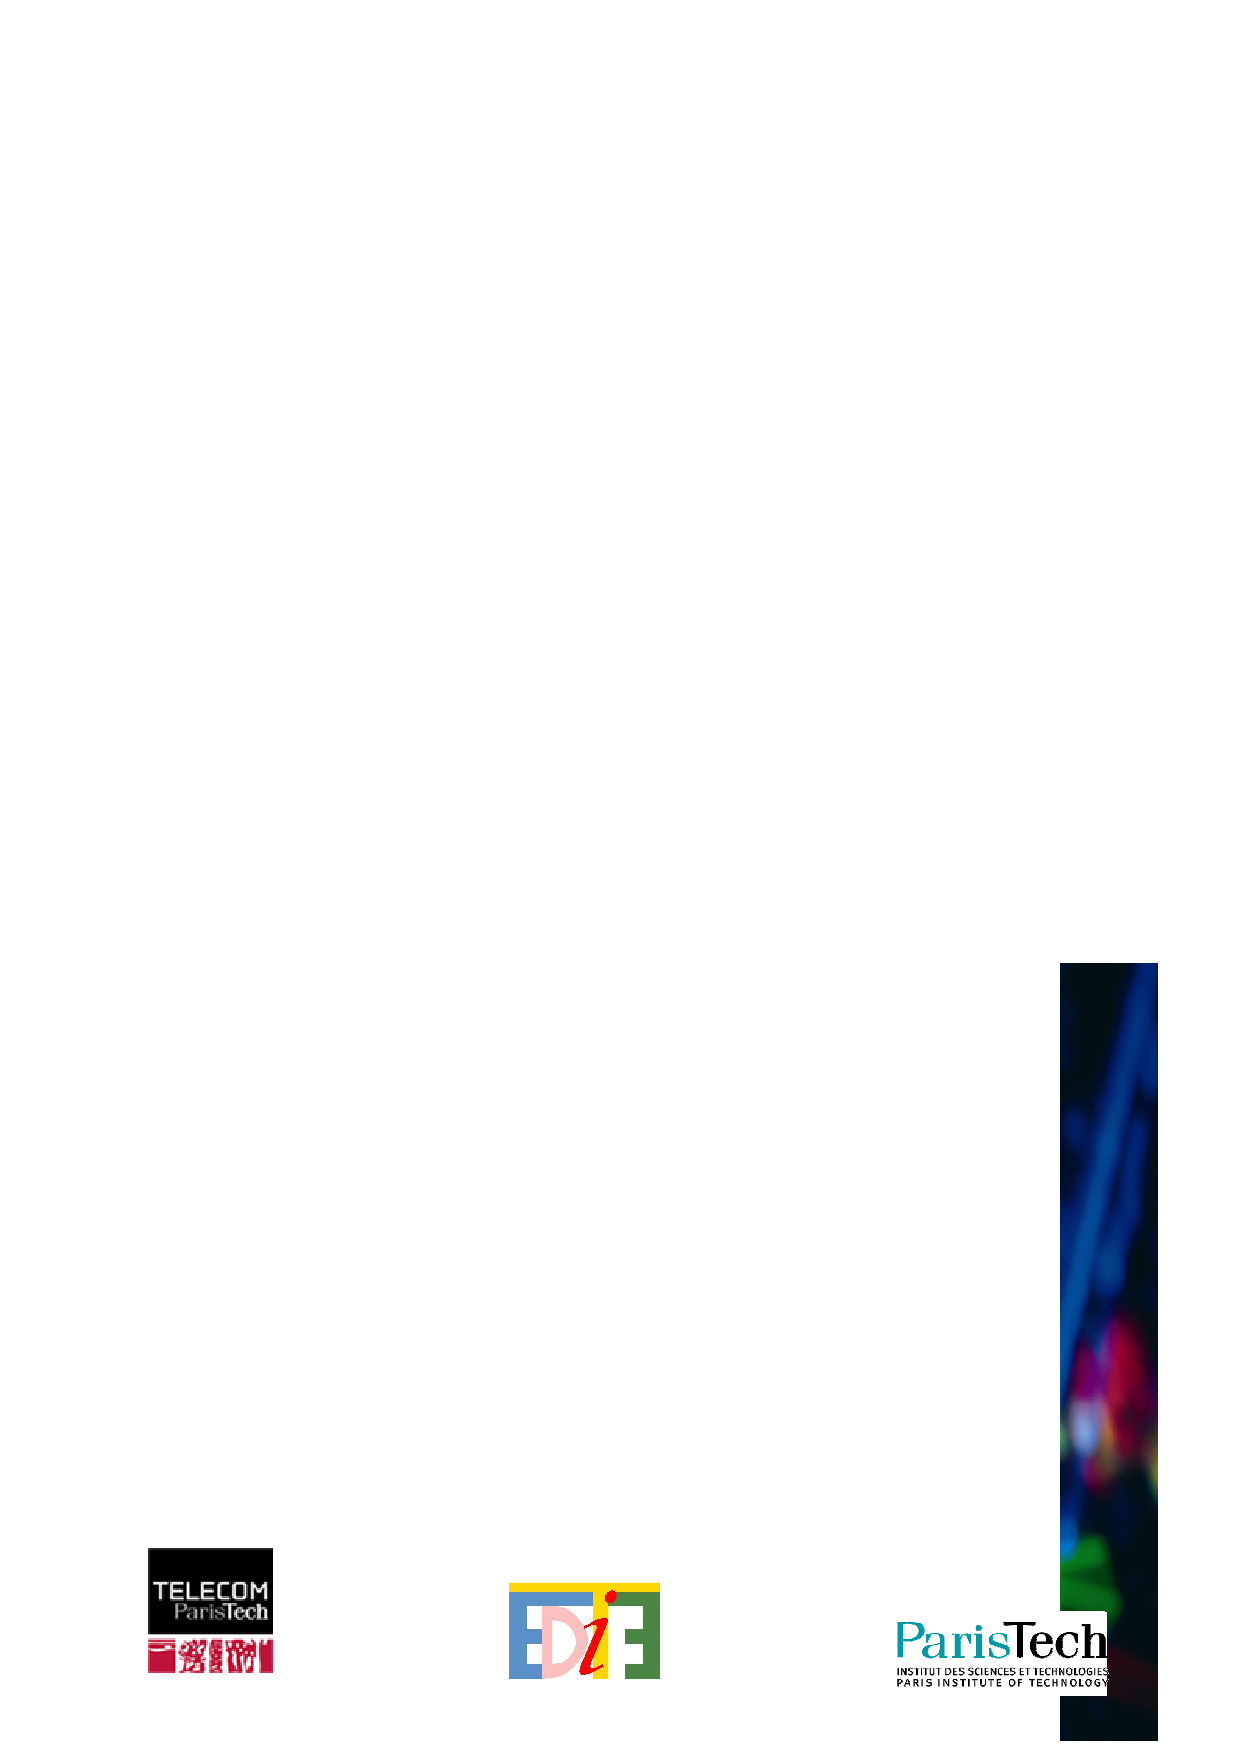
\includegraphics[height=\paperheight,width=\paperwidth]{cover_4_bg.pdf}
\else
%	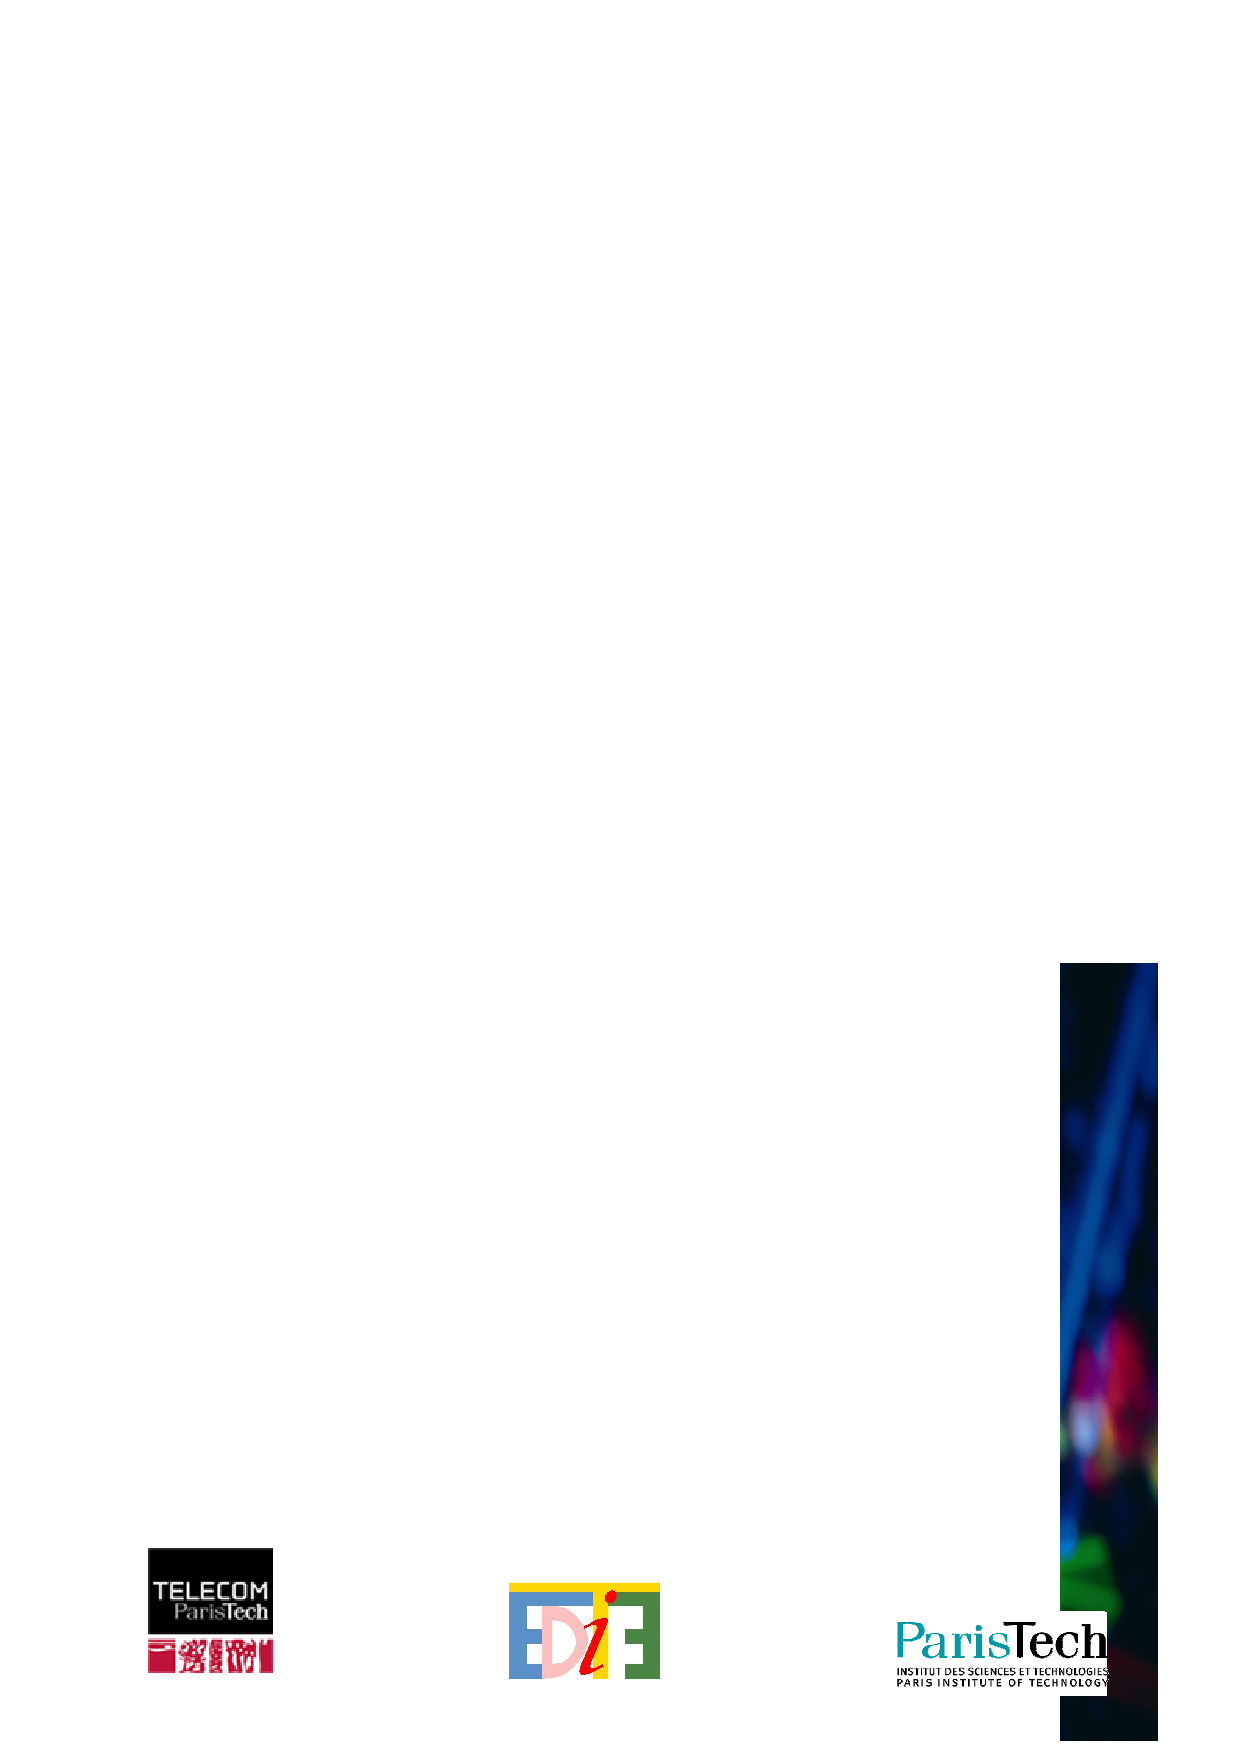
\includegraphics[height=\paperheight,width=\paperwidth]{cover_4_bg.pdf}
\fi
}

\pagestyle{empty}

\begin{document}
\AddToShipoutPicture*{\BackgroundPic}
~




%
\vspace{.5cm}
%

%
\vspace{1.0cm}
%
%
%
\begin{center}{\LARGE {\bf Validation of Security Protocols in Open and Mobile Environments}}\\
\vspace{.4cm}
{\large {\bf Trung NGUYEN}}\\
\end{center}

\vspace{.9cm}

{\bf RESUME : } r{\'e}sum{\'e} en fran{\,c}ais - r{\'e}sum{\'e} en fran{\,c}ais - r{\'e}sum{\'e} en fran{\,c}ais 
- r{\'e}sum{\'e} en fran{\,c}ais - r{\'e}sum{\'e} en fran{\,c}ais - r{\'e}sum{\'e} en fran{\,c}ais -r{\'e}sum{\'e} en fran{\,c}ais 
- r{\'e}sum{\'e} en fran{\,c}ais - r{\'e}sum{\'e} en fran{\,c}ais -r{\'e}sum{\'e} en fran{\,c}ais - r{\'e}sum{\'e} en fran{\,c}ais - r{\'e}sum{\'e} en fran{\,c}ais -

\vspace{.6cm}

{\bf MOTS-CLEFS:}  bla bla bla 

\vspace{1.0cm}

{\bf ABSTRACT: } 
A vital built-in feature of Internet of Thing is wireless communication which all devices work together wirelessly. Nevertheless this type of communication has brought major security challenges. One is device authentication that consists of several types of agreements such as time agreement, location agreement, or even connection agreement. These agreements have not been studied in traditional cryptographic protocols before since they strongly involve non-cryptographic properties. Furthermore, curent formal analysis partly subjects to such agreements. Understanding the obstacles, we study a new formal model that extends Strand Space model with physical characteristics and a stronger penetrator to help analyse existing wireless security protocols.

When studying device pairing protocols using our model, we found a flaw in a famous protocol proposed  by Wong \& Stajano using our model. This flaw has not been discovered before. Moreover in this work, we conduct a new secure and effective key agreement protocol between two wireless devices which offers better communication costs than other solutions, yet still ensures a reasonable security. Furthermore, we propose a translation procedure a model of an initial protocol with out-of-band channels into a model that does not use any out-of-band channel. The translation definitely preserves security properties of initial protocol. Straightforwardly, device pairing protocols can be automatically verified under existing tools. 

Our next contribution is analysing neighbor discovery protocols using our enhance models with notation of links, and useful supporting tools. During study security challenges of current neighbor discovery protocols, and formal methods for such protocols, we discover problems where time-based, and distance-based protocols cannot provide the exact link agreement on existence of principals in zone of their signal range. Several examples are illustrated as a proof of concept.

Based on above mentioned enhanced security protocols and our formal method, we conduct a new complete secure and robust bootstrapping scheme as our last contribution. The scheme enables a new resource constrained thing to securely join into a home network in some very sensitive circumstances. The circumstances are considered in this thesis is such that (1) the home gateway is down, or the thing is second-handed stuff, (2) things do not have pre-shared keys between things, or do not store public keys implanted at manufacture sites, (3) PKI system does not exists. Apparently, we also give clear formal proofs of security properties for our scheme. -
%

\vspace{.6cm}
{\bf KEY-WORDS: } Formal Model, Security Verification, Authentication Protocols, Strand Space
%
%
%
%


%
%
\end{document}
